\documentclass{beamer}
\usetheme{CambridgeUS}

\usepackage{graphicx}
\usepackage{subcaption}

\DeclareMathOperator*{\argmin}{argmin}

\title[GHSOM for Community Detection]{Growing Hierarchical Self Organising Maps for Community Detection}
\author{David McDonald}
\institute{University of Birmingham}
\date{23rd November 2016}

\begin{document}
	
	\begin{frame}
		\titlepage
	\end{frame}

	\begin{frame}{Recap}
		\begin{itemize}
			\item Using SOM to detect community structure in networks
			\item Most biological networks contain multi-scale (hierarchical) community structure 
		\end{itemize}
	\end{frame}

	\begin{frame}{Growing Hierarchical SOM (GHSOM)}
		\begin{itemize}
		\item using Growing Hierarchical SOM (GHSOM) to detect hierarchical community structure in complex networks 
		\item a variation of SOM, proposed in \cite{rauber2002growing} that can produce maps of arbitrary size and structure
		\item additionally, when the error of a neuron is large enough, that neuron is expanded into its own map, producing a hierarchical model
		\item like SOM, topological structure is preserved
		\end{itemize}
	\end{frame}

	\begin{frame}{Parameters}
	There are a few extra parameters in GHSOM than in standard SOM
		\begin{itemize}
			\item Mean Quantization Error of a map in layer $l$: $\textbf{MQE}_l$
			\item Mean Quantization Error of a single neuron $i$
			\item Stop map growth parameter: $e_{sg}$
			\begin{itemize}
				\item The error must fall below this times the previous levels error for growth to stop
				\item The smaller this is the larger the map will be
			\end{itemize}
			\item New layer parameter: $e_{en}$
			\begin{itemize}
				\item If the error of a single unit is greater than this times the error of the previous layer, then a new network will be constructed using the nodes connected to this unit
				\item The smaller this is, the deeper the network hierarchy
			\end{itemize}
		\end{itemize}
	\end{frame}

	\begin{frame}{GHSOM Algorithm}
		\begin{figure}
			\centering
			\includegraphics[width=\textwidth]{ghsom_diagram_presentation.png}
		\end{figure}
	\end{frame}
	
	\begin{frame}{Training}
%		\begin{figure}
%			\centering
%			\begin{subfigure}{width=\textwidth}
%				\centering
%				\includegraphics[width=\textwidth]{training_presentation.png}
%			\end{subfigure}%
%			
%			\begin{subfigure}{width=\textwidth}
%				\centering
%				\includegraphics[width=\textwidth]{grow_map_presentation.png}
%			\end{subfigure}
%
%
%		\end{figure}
	\begin{figure}
		\includegraphics[width=\textwidth]{training_presentation.png}
	\end{figure}
	\end{frame}
	
	\begin{frame}{Growing the map}
	\begin{figure}
	\includegraphics[width=\textwidth]{grow_map_presentation.png}
	\end{figure}	
	\end{frame}
	
	\begin{frame}{Adding a new layer}
	\begin{figure}
	\includegraphics[scale=0.35]{expand_presentation.png}
	\end{figure}	
	\end{frame}	
	
	\begin{frame}{Overall Algorithm}
		\begin{figure}
			\centering
			\includegraphics[width=\textwidth]{overall_algorithm_presentation.png}
		\end{figure}
	\end{frame}

	\begin{frame}{Example on Synthetic Benchmark graph}
	\begin{columns}
	\column{.45\textwidth}
		\begin{figure}
		\centering
		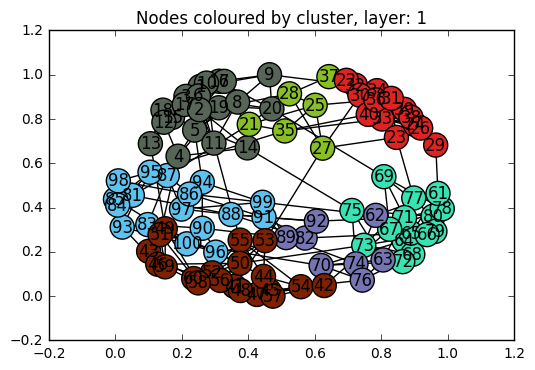
\includegraphics[scale=0.4]{benchmark.png}
		\end{figure}
	\column{.45\textwidth}
		\begin{figure}
		\centering
		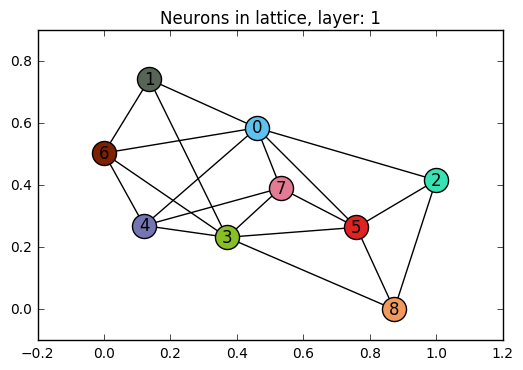
\includegraphics[scale=0.4]{map.png}
		\end{figure}
	\end{columns}
		Normalised mutual information score: 0.89584843255398483\\
		Notice the topological information about the communities is preserved \\
		Also, there are superfluous neurons (7)
	\end{frame}

	\begin{frame}{Next Steps}
		\begin{itemize}
			\item Obtain results on benchmark real world and synthetic datasets using Spearmint, Bayesian Optimisation software provided by Jasper Snoek et al. \cite{gelbart2014bayesian,snoek2014input,snoek2013bayesian}
			\item Finish literature review
			\item Write paper (hopefully!) for 19th February submission to IJCAI 2017 
		\end{itemize}
	\end{frame}
	
	\begin{frame}{What about afterwards?}
		\begin{itemize}
			\item Generative Topographical Map (probabilistic counterpart of SOM)
			\item Latent variable learning
			\begin{itemize}
				\item Boltzmann machine
				\item Autoencoders 
			\end{itemize}
			\item Use for Active module identification
		\end{itemize}
	\end{frame}

	\begin{frame}[allowframebreaks]{References}
		\bibliography{references}
		\bibliographystyle{unsrt}
	\end{frame}

\end{document}